% questions.tex —— 2021 年·全国乙卷·理科 · 题目内容片段（无答案）
% 由 tools/generate_projects.py 依来源总账自 2021/2021_数学真题_全国乙理_试题.md 生成，勿手改（改源 MD 后重跑）


\begin{gktip}
2021 普通高等学校招生考试（全国卷 I 理）
\end{gktip}

\par\medskip

\gkpart{一、选择题}

\begin{question}
\gkti{1}设 $2(z+\bar z)+3(z-\bar z)=4+6\mathrm i$，则 $z=$\mbox{（　　）}

\begin{gkopts}(4)
\task A．$1-2\mathrm i$
\task B．$1+2\mathrm i$
\task C．$1+\mathrm i$
\task D．$1-\mathrm i$
\end{gkopts}

\end{question}
\begin{question}
\gkti{2}已知集合 $S=\{s\mid s=2n+1,\ n\in\mathbf Z\}$，$T=\{t\mid t=4n+1,\ n\in\mathbf Z\}$，则 $S\cap T=$\mbox{（　　）}

\begin{gkopts}(4)
\task A．$\varnothing$
\task B．$S$
\task C．$T$
\task D．$\mathbf Z$
\end{gkopts}

\end{question}
\begin{question}
\gkti{3}已知命题 $p:\exists x\in\mathbf R,\ \sin x<1$；命题 $q:\forall x\in\mathbf R,\ \mathrm e^{|x|}\geqslant1$，则下列命题中为真命题的是\mbox{（　　）}

\begin{gkopts}(4)
\task A．$p\land q$
\task B．$\neg p\land q$
\task C．$p\land\neg q$
\task D．$\neg(p\lor q)$
\end{gkopts}

\end{question}
\begin{question}
\gkti{4}设函数 $f(x)=\dfrac{1-x}{1+x}$，则下列函数中是奇函数的是\mbox{（　　）}

\begin{gkopts}(4)
\task A．$f(x-1)-1$
\task B．$f(x-1)+1$
\task C．$f(x+1)-1$
\task D．$f(x+1)+1$
\end{gkopts}

\end{question}
\begin{question}
\gkti{5}在正方体 $ABCD-A_1B_1C_1D_1$ 中，$P$ 为 $B_1D_1$ 的中点，则直线 $PB$ 与 $AD_1$ 所成角为\mbox{（　　）}

\begin{gkopts}(4)
\task A．$\dfrac{\pi}{2}$
\task B．$\dfrac{\pi}{3}$
\task C．$\dfrac{\pi}{4}$
\task D．$\dfrac{\pi}{6}$
\end{gkopts}

\end{question}
\begin{question}
\gkti{6}将 $5$ 名北京冬奥会志愿者分配到花样滑冰、短道速滑、冰球和冰壶 $4$ 个项目进行培训，每名志愿者只分配到 $1$ 个项目，每个项目至少分配 $1$ 名志愿者，则不同的分配方案共有\mbox{（　　）}

\begin{gkopts}(4)
\task A．$60$ 种
\task B．$120$ 种
\task C．$240$ 种
\task D．$480$ 种
\end{gkopts}

\end{question}
\begin{question}
\gkti{7}把函数 $y=f(x)$ 图象上所有点的横坐标缩短到原来的 $\dfrac12$ 倍，纵坐标不变，再把所得曲线向右平移 $\dfrac{\pi}{3}$ 个单位长度，得到函数 $y=\sin\left(x-\dfrac{\pi}{4}\right)$ 的图象，则 $f(x)=$\mbox{（　　）}

\begin{gkopts}(1)
\task A．$\sin\left(\dfrac{x}{2}-\dfrac{7\pi}{12}\right)$
\task B．$\sin\left(\dfrac{x}{2}+\dfrac{\pi}{12}\right)$
\task C．$\sin\left(2x-\dfrac{7\pi}{12}\right)$
\task D．$\sin\left(2x+\dfrac{\pi}{12}\right)$
\end{gkopts}

\end{question}
\begin{question}
\gkti{8}在区间 $(0,1)$ 和 $(1,2)$ 中各随机取 $1$ 个数，则两数之和大于 $\dfrac74$ 的概率为\mbox{（　　）}

\begin{gkopts}(4)
\task A．$\dfrac79$
\task B．$\dfrac{23}{32}$
\task C．$\dfrac9{32}$
\task D．$\dfrac29$
\end{gkopts}

\Needspace{0.4\textheight}
\end{question}
\begin{question}
\gkti{9}魏晋时期刘徽编写的《海岛算经》是关于测量的数学著作，其中第一题是测量海岛的高。如图，点 $E,H,G$ 在水平线 $AC$ 上，$DE$ 和 $FG$ 是两个垂直于水平面且等高的测量标杆的高度，称为“表高”，$EG$ 称为“表距”，$GC$ 和 $EH$ 都称为“表目距”，$GC$ 与 $EH$ 的差称为“表目距的差”，则海岛的高 $AB=$\mbox{（　　）}
\nopagebreak[4]
\begin{center}% 2021 全国乙卷理科第 9 题：海岛测高示意图；逻辑图名 2021-national-b-science-t09-island
% 依据 PDF 第 1 页；A、E、H、G、C 共线，DE=FG，B-D-H 与 B-F-C 共线。
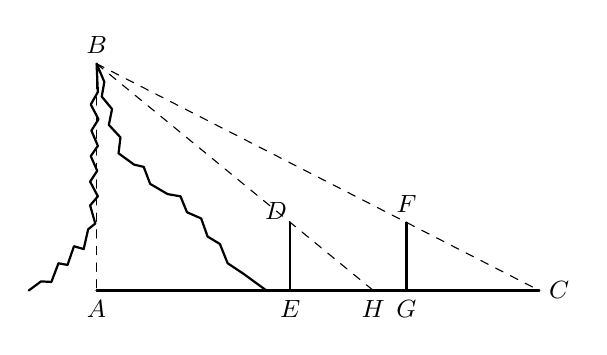
\begin{tikzpicture}[x=0.82cm,y=0.72cm,line cap=round,line join=round,font=\small]
  \coordinate (A) at (0,0);
  \coordinate (B) at (0,4);
  \coordinate (E) at (3,0);
  \coordinate (D) at (3,1.2);
  \coordinate (H) at (4.286,0);
  \coordinate (G) at (4.8,0);
  \coordinate (F) at (4.8,1.2);
  \coordinate (C) at (6.857,0);

  % Island outline and measured height
  \draw[thick]
    (-1.05,0) -- (-0.86,0.16) -- (-0.70,0.15) -- (-0.59,0.48)
    -- (-0.45,0.45) -- (-0.35,0.78) -- (-0.20,0.73) -- (-0.13,1.08)
    -- (-0.02,1.18) -- (-0.10,1.50) -- (0.02,1.66) -- (-0.10,1.92)
    -- (0.01,2.11) -- (-0.09,2.37) -- (0.02,2.55) -- (-0.08,2.82)
    -- (0.03,3.02) -- (-0.09,3.28) -- (0.02,3.50) -- (0,4)
    -- (0.12,3.68) -- (0.08,3.42) -- (0.24,3.20) -- (0.19,2.92)
    -- (0.37,2.70) -- (0.34,2.42) -- (0.58,2.22) -- (0.73,2.18)
    -- (0.83,1.88) -- (1.10,1.70) -- (1.30,1.66) -- (1.40,1.38)
    -- (1.62,1.27) -- (1.72,0.95) -- (1.91,0.82) -- (2.03,0.48)
    -- (2.28,0.29) -- (2.63,0);
  \draw[dashed] (B) -- (A);

  % Horizontal reference line, equal poles and sight lines
  \draw[thick] (A) -- (C);
  \draw[dashed] (B) -- (H);
  \draw[dashed] (B) -- (C);
  \draw[thick] (D) -- (E);
  \draw[thick] (F) -- (G);

  \node[above] at (B) {$B$};
  \node[below] at (A) {$A$};
  \node[above left,inner sep=1pt] at (D) {$D$};
  \node[below] at (E) {$E$};
  \node[below] at (H) {$H$};
  \node[above] at (F) {$F$};
  \node[below] at (G) {$G$};
  \node[right] at (C) {$C$};
\end{tikzpicture}
\end{center}
\nopagebreak[4]
\begin{gkopts}(1)
\task A．$\dfrac{\text{\text{表高}}\times\text{\text{表距}}}{\text{\text{表目距的差}}}+\text{\text{表高}}$
\task B．$\dfrac{\text{\text{表高}}\times\text{\text{表距}}}{\text{\text{表目距的差}}}-\text{\text{表高}}$
\task C．$\dfrac{\text{\text{表高}}\times\text{\text{表距}}}{\text{\text{表目距的差}}}+\text{\text{表距}}$
\task D．$\dfrac{\text{\text{表高}}\times\text{\text{表距}}}{\text{\text{表目距的差}}}-\text{\text{表距}}$
\end{gkopts}

\end{question}
\begin{question}
\gkti{10}设 $a\ne0$，若 $x=a$ 是函数 $f(x)=a(x-a)^2(x-b)$ 的极大值点，则\mbox{（　　）}

\begin{gkopts}(4)
\task A．$a<b$
\task B．$a>b$
\task C．$ab<a^2$
\task D．$ab>a^2$
\end{gkopts}

\end{question}
\begin{question}
\gkti{11}设 $B$ 是椭圆 $C:\dfrac{x^2}{a^2}+\dfrac{y^2}{b^2}=1\ (a>b>0)$ 的上顶点，若 $C$ 上任意一点 $P$ 都满足 $|PB|\leqslant2b$，则 $C$ 的离心率的取值范围是\mbox{（　　）}

\begin{gkopts}(2)
\task A．$\left[\dfrac{\sqrt2}{2},1\right)$
\task B．$\left[\dfrac12,1\right)$
\task C．$\left(0,\dfrac{\sqrt2}{2}\right]$
\task D．$\left(0,\dfrac12\right]$
\end{gkopts}

\end{question}
\begin{question}
\gkti{12}设 $a=2\ln1.01$，$b=\ln1.02$，$c=\sqrt{1.04}-1$，则\mbox{（　　）}

\begin{gkopts}(4)
\task A．$a<b<c$
\task B．$b<c<a$
\task C．$b<a<c$
\task D．$c<a<b$
\end{gkopts}

\par\medskip

\end{question}
\gkpart{二、填空题}

\begin{question}
\gkti{13}已知双曲线 $C:\dfrac{x^2}{m}-y^2=1\ (m>0)$ 的一条渐近线为 $\sqrt3x+my=0$，则 $C$ 的焦距为 $\underline{\qquad\qquad}$．

\end{question}
\begin{question}
\gkti{14}已知向量 $\boldsymbol a=(1,3)$，$\boldsymbol b=(3,4)$，$(\boldsymbol a-\lambda\boldsymbol b)\perp\boldsymbol b$，则 $\lambda=$ $\underline{\qquad\qquad}$．

\end{question}
\begin{question}
\gkti{15}记 $\triangle ABC$ 的内角 $A,B,C$ 的对边分别为 $a,b,c$，面积为 $\sqrt3$，$B=60^\circ$，$a^2+c^2=3ac$，则 $b=$ $\underline{\qquad\qquad}$．

\Needspace{0.4\textheight}
\end{question}
\begin{question}
\gkti{16}以图①为正视图，在图②③④⑤中选两个分别作为侧视图和俯视图，组成某个三棱锥的三视图，则所选侧视图和俯视图的编号依次为 $\underline{\qquad\qquad}$．（写出符合要求的一组答案即可）
\nopagebreak[4]
\begin{center}% 2021 全国乙卷理科第 16 题：正视图与候选侧视图、俯视图；逻辑图名 2021-national-b-science-t16-views
\begin{tikzpicture}[x=0.72cm,y=0.72cm,line cap=round,line join=round,font=\small]
  % Front view (figure 1)
  \coordinate (a1) at (0,0);
  \coordinate (b1) at (2,0);
  \coordinate (c1) at (2,1);
  \draw[thick] (a1) -- (b1) -- (c1) -- cycle;
  \draw (0,-0.08) -- (0,-0.30);
  \draw (2,-0.08) -- (2,-0.30);
  \draw[<->] (0,-0.25) -- (2,-0.25) node[midway,below,inner sep=1pt] {$2$};
  \draw (2.08,0) -- (2.34,0);
  \draw (2.08,1) -- (2.34,1);
  \draw[<->] (2.27,0) -- (2.27,1) node[midway,right,inner sep=1pt] {$1$};
  \node[below] at (1,-0.62) {图①};

  % Side-view option 2: visible central edge
  \coordinate (a2) at (3.45,0);
  \coordinate (b2) at (5.45,0);
  \coordinate (c2) at (4.45,1);
  \draw[thick] (a2) -- (b2) -- (c2) -- cycle;
  \draw[thick] (c2) -- (4.45,0);
  \draw (3.45,-0.08) -- (3.45,-0.30);
  \draw (5.45,-0.08) -- (5.45,-0.30);
  \draw[<->] (3.45,-0.25) -- (5.45,-0.25) node[midway,below,inner sep=1pt] {$2$};
  \draw (5.53,0) -- (5.78,0);
  \draw (5.53,1) -- (5.78,1);
  \draw[<->] (5.72,0) -- (5.72,1) node[midway,right,inner sep=1pt] {$1$};
  \node[below] at (4.45,-0.62) {图②};

  % Side-view option 3: hidden central edge
  \coordinate (a3) at (7.05,0);
  \coordinate (b3) at (9.05,0);
  \coordinate (c3) at (8.05,1);
  \draw[thick] (a3) -- (b3) -- (c3) -- cycle;
  \draw[dashed] (c3) -- (8.05,0);
  \draw (7.05,-0.08) -- (7.05,-0.30);
  \draw (9.05,-0.08) -- (9.05,-0.30);
  \draw[<->] (7.05,-0.25) -- (9.05,-0.25) node[midway,below,inner sep=1pt] {$2$};
  \draw (9.13,0) -- (9.38,0);
  \draw (9.13,1) -- (9.38,1);
  \draw[<->] (9.32,0) -- (9.32,1) node[midway,right,inner sep=1pt] {$1$};
  \node[below] at (8.05,-0.62) {图③};

  % Top-view options are shifted down to keep their geometry clear of the upper-row labels.
  \begin{scope}[yshift=-0.5cm]
  % Top-view option 4
  \coordinate (a4) at (0,-2.65);
  \coordinate (b4) at (0,-0.65);
  \coordinate (c4) at (2,-1.65);
  \draw[thick] (a4) -- (b4) -- (c4) -- cycle;
  \draw (-0.08,-2.65) -- (-0.34,-2.65);
  \draw (-0.08,-0.65) -- (-0.34,-0.65);
  \draw[<->] (-0.27,-2.65) -- (-0.27,-0.65) node[midway,left,inner sep=1pt] {$2$};
  \draw (0,-2.73) -- (0,-2.96);
  \draw (2,-1.73) -- (2,-2.96);
  \draw[<->] (0,-2.88) -- (2,-2.88) node[midway,below,inner sep=1pt] {$2$};
  \node[below] at (1,-3.22) {图④};

  % Top-view option 5, with the visible median
  \coordinate (a5) at (5.25,-0.65);
  \coordinate (b5) at (5.25,-2.65);
  \coordinate (c5) at (3.25,-1.65);
  \draw[thick] (a5) -- (b5) -- (c5) -- cycle;
  \draw[thick] (c5) -- (5.25,-1.65);
  \draw (5.33,-2.65) -- (5.58,-2.65);
  \draw (5.33,-0.65) -- (5.58,-0.65);
  \draw[<->] (5.50,-2.65) -- (5.50,-0.65) node[midway,right,inner sep=1pt] {$2$};
  \draw (3.25,-1.73) -- (3.25,-2.96);
  \draw (5.25,-2.73) -- (5.25,-2.96);
  \draw[<->] (3.25,-2.88) -- (5.25,-2.88) node[midway,below,inner sep=1pt] {$2$};
  \node[below] at (4.25,-3.22) {图⑤};
  \end{scope}
\end{tikzpicture}
\end{center}
\nopagebreak[4]
\par\medskip

\end{question}
\gkpart{三、解答题}

\begin{question}
\gkti{17}某厂研制了一种生产高精产品的设备，为检验新设备生产产品的某项指标有无提高，用一台旧设备和一台新设备各生产了 $10$ 件产品，得到各件产品该项指标数据如下：

\begin{center}
\begingroup\setlength{\tabcolsep}{4pt}
\begin{tabular}{crrrrrrrrrr}
\toprule
设备 & 1 & 2 & 3 & 4 & 5 & 6 & 7 & 8 & 9 & 10 \\
\midrule
旧设备 & $9.8$ & $10.3$ & $10.0$ & $10.2$ & $9.9$ & $9.8$ & $10.0$ & $10.1$ & $10.2$ & $9.7$ \\
新设备 & $10.1$ & $10.4$ & $10.1$ & $10.0$ & $10.1$ & $10.3$ & $10.6$ & $10.5$ & $10.4$ & $10.5$ \\
\bottomrule
\end{tabular}
\endgroup
\end{center}

旧设备和新设备生产产品的该项指标的样本平均值分别记为 $\bar x$ 和 $\bar y$，样本方差分别记为 $s_1^2$ 和 $s_2^2$。

  (1) 求 $\bar x,\bar y,s_1^2,s_2^2$；

  (2) 判断新设备生产产品的该项指标的均值较旧设备是否有显著提高（如果 $\bar y-\bar x\geqslant2\sqrt{\dfrac{s_1^2+s_2^2}{10}}$，则认为新设备生产产品的该项指标的均值较旧设备有显著提高，否则不认为有显著提高）．

\Needspace{0.4\textheight}
\end{question}
\begin{question}
\gkti{18}如图，四棱锥 $P-ABCD$ 的底面是矩形，$PD\perp$ 底面 $ABCD$，$PD=DC=1$，$M$ 为 $BC$ 的中点，且 $PB\perp AM$。
\nopagebreak[4]
\begin{center}% 2021 全国乙卷理科第 18 题：四棱锥 P-ABCD，底面 ABCD 为矩形；逻辑图名 2021-national-b-science-t18-pyramid
% 隐藏棱 AD、DC、PD 以虚线表示；M 为 BC 中点，连结 PM。
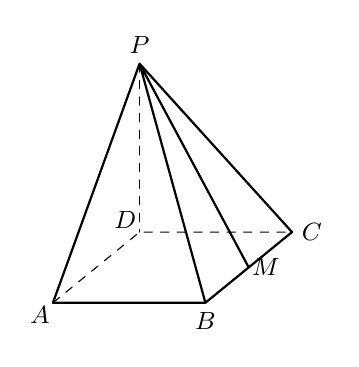
\begin{tikzpicture}[x=0.88cm,y=0.88cm,line cap=round,line join=round,font=\small]
  \coordinate (A) at (0,0);
  \coordinate (B) at (2.2,0);
  \coordinate (C) at (3.45,1.02);
  \coordinate (D) at (1.25,1.02);
  \coordinate (P) at (1.25,3.45);
  \coordinate (M) at (2.825,0.51);

  % Visible base and lateral edges
  \draw[thick] (A) -- (B) -- (C);
  \draw[thick] (P) -- (A) (P) -- (B) (P) -- (C) (P) -- (M);

  % Hidden rear edges
  \draw[dashed] (A) -- (D) -- (C);
  \draw[dashed] (P) -- (D);

  \node[above] at (P) {$P$};
  \node[below left,inner sep=1pt] at (A) {$A$};
  \node[below] at (B) {$B$};
  \node[right] at (C) {$C$};
  \node[above left,inner sep=1pt] at (D) {$D$};
  \node[right,inner sep=1pt] at (M) {$M$};
\end{tikzpicture}
\end{center}
\nopagebreak[4]
  (1) 求 $BC$；

  (2) 求二面角 $A-PM-B$ 的正弦值。

\end{question}
\begin{question}
\gkti{19}记 $S_n$ 为数列 $\{a_n\}$ 的前 $n$ 项和，$b_n$ 为数列 $\{S_n\}$ 的前 $n$ 项积，已知 $\dfrac2{S_n}+\dfrac1{b_n}=2$。

  (1) 证明：数列 $\{b_n\}$ 是等差数列；

  (2) 求 $\{a_n\}$ 的通项公式。

\end{question}
\begin{question}
\gkti{20}设函数 $f(x)=\ln(a-x)$，已知 $x=0$ 是函数 $y=xf(x)$ 的极值点。

  (1) 求 $a$；

  (2) 设函数 $g(x)=\dfrac{x+f(x)}{xf(x)}$，证明：$g(x)<1$。

\end{question}
\begin{question}
\gkti{21}已知抛物线 $C:x^2=2py\ (p>0)$ 的焦点为 $F$，且 $F$ 与圆 $M:x^2+(y+4)^2=1$ 上的点的距离的最小值为 $4$。

  (1) 求 $p$；

  (2) 若点 $P$ 在圆 $M$ 上，$PA,PB$ 是 $C$ 的两条切线，$A,B$ 是切点，求 $\triangle PAB$ 面积的最大值。

\end{question}
\begin{question}
\gkti{22}在直角坐标系 $xOy$ 中，$\odot C$ 的圆心为 $C(2,1)$，半径为 $1$。

  (1) 写出 $\odot C$ 的一个参数方程；

  (2) 过点 $F(4,1)$ 作 $\odot C$ 的两条切线，以坐标原点为极点，$x$ 轴正半轴为极轴建立极坐标系，求这两条切线的极坐标方程。

\end{question}
\begin{question}
\gkti{23}已知函数 $f(x)=|x-a|+|x+3|$。

  (1) 当 $a=1$ 时，求不等式 $f(x)\geqslant6$ 的解集；

  (2) 若 $f(x)>-a$，求 $a$ 的取值范围。

\makeatletter\def\gkanswerblock{answer}\ifx\@currenvir\gkanswerblock\else\clearpage\fi\makeatother

\end{question}